\documentclass[a4paper,11pt]{article}
\usepackage[utf8]{inputenc}\usepackage[T1]{fontenc}
\usepackage[english]{babel}\usepackage{lmodern}\usepackage{microtype}
\usepackage{amsmath,amssymb}\usepackage{geometry}
\geometry{a4paper,left=2.2cm,right=2.2cm,top=2.0cm,bottom=2.0cm}
\usepackage{booktabs,array}\usepackage{xcolor}
\definecolor{bokug}{RGB}{0,135,60}\usepackage{tikz}
\usetikzlibrary{arrows.meta,calc}
\usepackage{fancyhdr}\pagestyle{fancy}
\renewcommand{\headrulewidth}{0.4pt}
\usepackage{enumitem}\setlength{\parindent}{0pt}\setlength{\parskip}{4pt}

\begin{document}
\fancyhead[L]{\small VU Mechanik – LAWI 100515 (PI)}\fancyhead[R]{\small SS 2026}\fancyfoot[C]{\thepage}
\begin{center}{\large\bfseries\color{bokug}University of Natural Resources and Life Sciences, Vienna (BOKU)}\\[2pt]{\large\bfseries VU Mechanik – LAWI 100515 (PI)}\\[4pt]Exam \textbf{Group A} \hfill Date: 26.06.2026\\[2pt]\rule{\linewidth}{0.4pt}\end{center}

\textbf{Given system}\par The planar system consists of bending beams and a truss connected by hinges.
\begin{center}
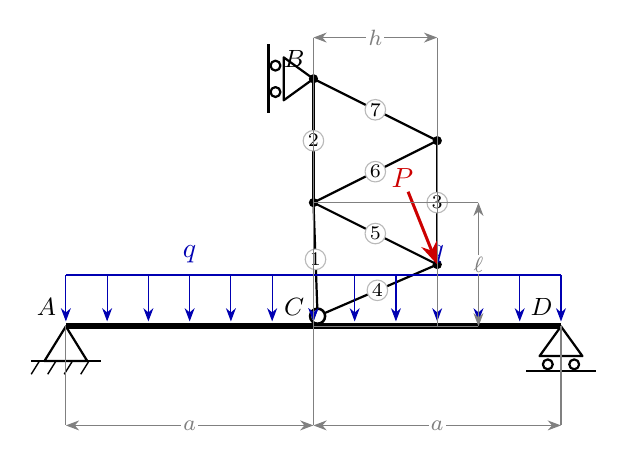
\begin{tikzpicture}[scale=1.048,>=Stealth,line join=round]
  \coordinate (P0) at (0.000,0.000);
  \coordinate (P1) at (3.000,0.000);
  \coordinate (P2) at (6.000,0.000);
  \coordinate (TO1) at (3.000,1.500);
  \coordinate (TO2) at (3.000,3.000);
  \coordinate (TU0) at (4.500,0.750);
  \coordinate (TU1) at (4.500,2.250);
  \coordinate (CPIN) at (3.050,0.124);
  \draw[thick] (CPIN) -- (TO1);
  \draw[thick] (TO1) -- (TO2);
  \draw[thick] (TU0) -- (TU1);
  \draw[thick] (CPIN) -- (TU0);
  \draw[thick] (TU0) -- (TO1);
  \draw[thick] (TO1) -- (TU1);
  \draw[thick] (TU1) -- (TO2);
  \draw[line width=2.2pt] (P0) -- (P1);
  \draw[line width=2.2pt] (P1) -- (P2);
  \fill (TO1) circle (1.6pt);
  \fill (TO2) circle (1.6pt);
  \fill (TU0) circle (1.6pt);
  \fill (TU1) circle (1.6pt);
  \draw[fill=white,line width=0.9pt] (CPIN) circle (2.6pt);
  \draw[thick] (0.000,0.000) -- (-0.260,-0.420) -- (0.260,-0.420) -- cycle;
  \draw[line width=1pt] (-0.420,-0.420) -- (0.420,-0.420);
  \draw[line width=0.5pt] (-0.320,-0.420) -- (-0.420,-0.580);
  \draw[line width=0.5pt] (-0.120,-0.420) -- (-0.220,-0.580);
  \draw[line width=0.5pt] (0.080,-0.420) -- (-0.020,-0.580);
  \draw[line width=0.5pt] (0.280,-0.420) -- (0.180,-0.580);
  \draw[thick] (6.000,0.000) -- (5.740,-0.360) -- (6.260,-0.360) -- cycle;
  \draw[thick] (5.840,-0.460) circle (0.06) (6.160,-0.460) circle (0.06);
  \draw[line width=1pt] (5.580,-0.540) -- (6.420,-0.540);
  \draw[thick] (3.000,3.000) -- (2.640,3.260) -- (2.640,2.740) -- cycle;
  \draw[thick] (2.540,3.160) circle (0.06) (2.540,2.840) circle (0.06);
  \draw[line width=1pt] (2.460,3.420) -- (2.460,2.580);
  \node[circle,fill=white,draw=gray!55,inner sep=0.5pt,font=\scriptsize] at (3.025,0.812) {1};
  \node[circle,fill=white,draw=gray!55,inner sep=0.5pt,font=\scriptsize] at (3.000,2.250) {2};
  \node[circle,fill=white,draw=gray!55,inner sep=0.5pt,font=\scriptsize] at (4.500,1.500) {3};
  \node[circle,fill=white,draw=gray!55,inner sep=0.5pt,font=\scriptsize] at (3.775,0.437) {4};
  \node[circle,fill=white,draw=gray!55,inner sep=0.5pt,font=\scriptsize] at (3.750,1.125) {5};
  \node[circle,fill=white,draw=gray!55,inner sep=0.5pt,font=\scriptsize] at (3.750,1.875) {6};
  \node[circle,fill=white,draw=gray!55,inner sep=0.5pt,font=\scriptsize] at (3.750,2.625) {7};
  \draw[->,blue!70!black] (0.000,0.620) -- (0.000,0.060);
  \draw[->,blue!70!black] (0.500,0.620) -- (0.500,0.060);
  \draw[->,blue!70!black] (1.000,0.620) -- (1.000,0.060);
  \draw[->,blue!70!black] (1.500,0.620) -- (1.500,0.060);
  \draw[->,blue!70!black] (2.000,0.620) -- (2.000,0.060);
  \draw[->,blue!70!black] (2.500,0.620) -- (2.500,0.060);
  \draw[->,blue!70!black] (3.000,0.620) -- (3.000,0.060);
  \draw[blue!70!black,thick] (0.000,0.620) -- (3.000,0.620);
  \node[blue!70!black] at (1.500,0.870) {$q$};
  \draw[->,blue!70!black] (3.000,0.620) -- (3.000,0.060);
  \draw[->,blue!70!black] (3.500,0.620) -- (3.500,0.060);
  \draw[->,blue!70!black] (4.000,0.620) -- (4.000,0.060);
  \draw[->,blue!70!black] (4.500,0.620) -- (4.500,0.060);
  \draw[->,blue!70!black] (5.000,0.620) -- (5.000,0.060);
  \draw[->,blue!70!black] (5.500,0.620) -- (5.500,0.060);
  \draw[->,blue!70!black] (6.000,0.620) -- (6.000,0.060);
  \draw[blue!70!black,thick] (3.000,0.620) -- (6.000,0.620);
  \node[blue!70!black] at (4.500,0.870) {$q$};
  \draw[->,red!80!black,line width=1.1pt] (4.147,1.632) -- (4.500,0.750);
  \node[red!80!black] at (4.080,1.799) {$P$};
  \draw[thin,gray] (0.000,0.000) -- (0.000,-1.200);
  \draw[thin,gray] (3.000,0.000) -- (3.000,-1.200);
  \draw[<->,gray] (0.000,-1.200) -- (3.000,-1.200) node[midway,fill=white,inner sep=0.8pt,font=\footnotesize]{$a$};
  \draw[thin,gray] (3.000,0.000) -- (3.000,-1.200);
  \draw[thin,gray] (6.000,0.000) -- (6.000,-1.200);
  \draw[<->,gray] (3.000,-1.200) -- (6.000,-1.200) node[midway,fill=white,inner sep=0.8pt,font=\footnotesize]{$a$};
  \draw[thin,gray] (3.000,0.000) -- (5.000,0.000);
  \draw[thin,gray] (3.000,1.500) -- (5.000,1.500);
  \draw[<->,gray] (5.000,0.000) -- (5.000,1.500) node[midway,fill=white,inner sep=0.8pt,font=\footnotesize]{$\ell$};
  \draw[thin,gray] (3.000,0.000) -- (3.000,3.500);
  \draw[thin,gray] (4.500,0.000) -- (4.500,3.500);
  \draw[<->,gray] (3.000,3.500) -- (4.500,3.500) node[midway,fill=white,inner sep=0.8pt,font=\footnotesize]{$h$};
  \node[font=\small] at (0.000,0.000) [xshift=-7pt,yshift=7pt] {$A$};
  \node[font=\small] at (3.000,0.000) [xshift=-7pt,yshift=7pt] {$C$};
  \node[font=\small] at (6.000,0.000) [xshift=-7pt,yshift=7pt] {$D$};
  \node[font=\small] at (3.000,3.000) [xshift=-7pt,yshift=7pt] {$B$};
\end{tikzpicture}
\end{center}
\textbf{Given quantities:}\quad $a=3$\,m\quad $\ell=1,5$\,m\quad $h=1,5$\,m\quad $q=4$\,kN/m\quad $P=20$\,kN
\par\medskip
\textbf{Tasks}\par
\begin{enumerate}[label=\textbf{\arabic*.}]
  \item Determine the degree of static determinacy.
  \item Compute all support reactions and hinge forces.
  \item Determine all truss member forces (tension/compression).
  \item Draw the section forces $N$, $V$, $M$ of the bending beams.
\end{enumerate}
\end{document}